\chapter{Information Visualization}

\label{chap:InfoVis}

Information visualization is the science of representing abstract information as interactive graphics to present and analyze it more efficiently. These two goals of presenting and analyzing abstract information in a visual form are built on the properties of human visual perception, which include the rapid scanning, recognition and recollection of visual information as well as the automatic detection of patterns in it. In contrast to textual representations of data, the processing of well-designed visualizations requires much less cognitive effort because it leverages features of the human visual processing system such as preattentive processing, meaning that certain visual attributes can be processed very quickly and without any conscious effort \parencite{PreattentiveProcessing}. 

In addition to visuals being easier to assimilate by humans, a purely textual and statistical view on data can also lead to erroneous assumptions as demonstrated by \cite{AnscombesQuartet} in the infamous visualization of four completely different datasets that have identical summary statistics, called Anscombe's Quartet. An observer trying to understand these sets of data purely from their statistics would mistakenly deem them to be identical because their inequality will only become obvious after carefully examining and comparing the individual entries in the datasets themselves, which is a tedious and error-prone task when not aided by visual representations like Figure \ref{fig:AnscombesQuartet}. Even though Anscombe's Quartet is very likely the most famous example to demonstrate this characteristic, it is certainly not the only set of datasets that possesses it, as has been shown by \cite{GenDataIdenticalStatisticsDissimilarGraphics}.

\begin{figure}[tp]
    \centering
    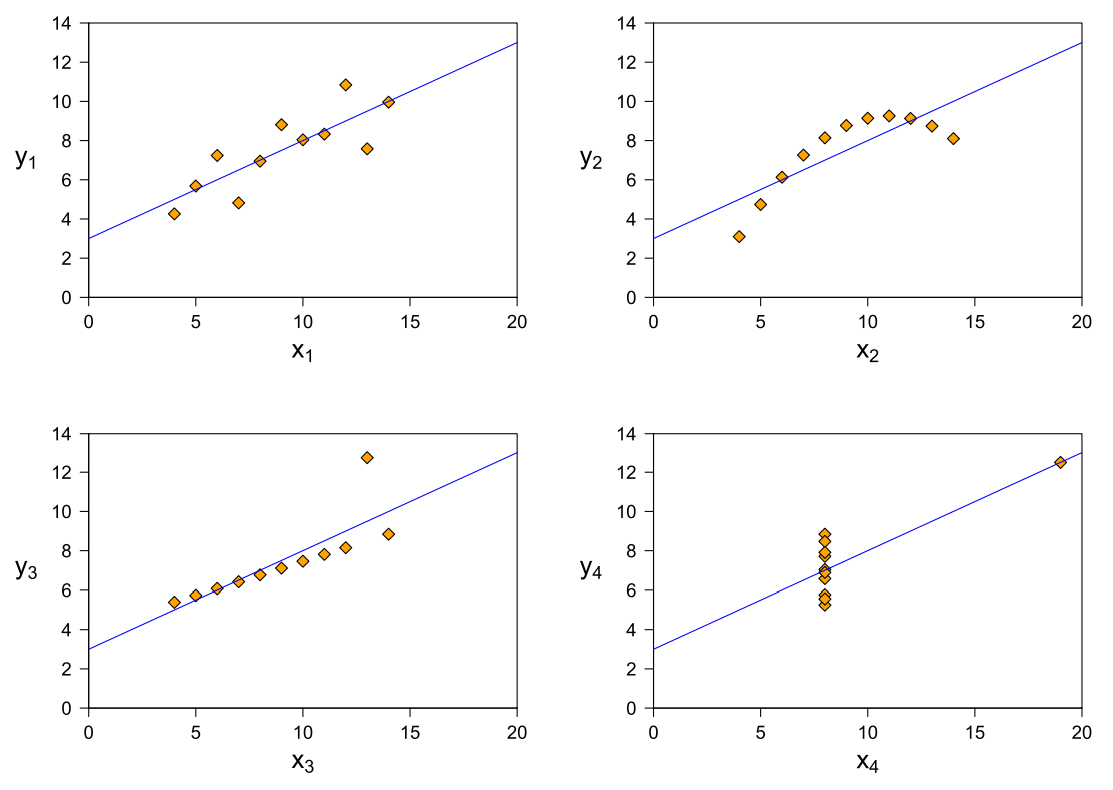
\includegraphics[keepaspectratio,width=\linewidth,height=\fullh / 2]
    {images/anscombes-quartet.png}

    \caption[Anscombe's Quartet]{
        Anscombe's Quartet consists of four distinct sets of data that share identical summary statistics. The difference between these datasets is only obvious by carefully examining the textual data or by plotting it. \imgcredit{Image extracted from \cite{IVISCourseNotes}. \TODO{Clarify how to credit correctly or recreate graphic}}
    }
    \label{fig:AnscombesQuartet}
\end{figure}

Regarding terminology, this work adheres to the separation of the field of visualization into three main subfields as described by \cite{IVISCourseNotes}: 

\begin{enumerate}
    \item Information Visualization: Deals with abstract data, which has no inherent presentation and for which a suitable type of visualization has to be chosen.
    \item Geographic Visualization: Deals with map-based data that has an inherent spatial dimension. 
    \item Scientific Visualization: Deals with object-related data that has inherent presentation, which is usually related to the object's real world representation.
\end{enumerate}

In addition to these three subfields, \cite{IVISCourseNotes} defines the often used term Data Visualization as the intersection of Geographic Visualization and Information Visualization. Therefore, it deals with visualizing spatial as well as abstract data.

Visualizations presented in an interactive medium do not merely consist of visual representations. In order to analyze more complex datasets, it is equally important to provide means for interacting with these representations because without interaction, a visualization becomes a static image, which has only very limited usefulness when dealing with large and multidimensional data. Even though the majority of the attention in the field of Information Visualization has been put on the presentational aspect of visualizations, a lot of research has also been conducted on their interactive aspects. Many taxonomies have been formulated with the goal of defining the design space of interactions to support analytic reasoning, but they vary greatly depending on the concepts they are focusing on. Some taxonomies have been defined on the concept of low-level interaction techniques \parencite{TheEyesHaveIt,GrammarOfGraphics}, providing a very system-centric view on interaction, while other taxonomies focus on user tasks \parencite{LowLevelComponentsOfAnalyticActivity} without them being tightly bound to interacting with visualizations. \cite{RoleOfInteractionInInformationVisualization} aims to provide a view that is in between the purely system-centric and purely user-centric extremes by defining a taxonomy based on user intent. The categories of this taxonomy are listed in Table \ref{tab:UserIntentCategories}, and they form a good framework with which interactivity in the context of Information Visualization can be discussed. 

\begin{table}[tp]
    \centering
    \begin{tabularx}{\linewidth}{| l | X | X |}
        \hline
        \textbf{Category} & \textbf{Description} & \textbf{Examples} \\ \hline
        Select & Mark items as interesting. &  \\ \hline
        Explore & Show different items. & Panning, direct-walk  \\ \hline
        Reconfigure & Show a different arrangement. & Dimension configuration, position adjustments \\ \hline
        Encode & Show a different representation. & Change chart type, orientation, colors, shapes, ... \\ \hline
        Abstract/Elaborate & Show more or less detail. & Details-on-demand (drill-down, sunburst, tooltips, zooming)  \\ \hline
        Filter & Show items based on conditions. & Dynamic query controls   \\ \hline
        Connect & Show related items. & Highlight connected items, highlight item in different representations   \\ \hline
        
    \end{tabularx}
    \caption[Categories of Interaction Based on User Intent]
    {
        This table shows the different categories of interacting with visualizations based on user intent.
        \imgcredit{Table created by the author of this thesis with data from \cite{RoleOfInteractionInInformationVisualization}}
    }
    \label{tab:UserIntentCategories}
\end{table}

The history of Information Visualization goes back a long time with one of the earliest examples dating back to the 10th century, when an unknown astronomer created a chart about the movement of the most prominent planets \parencite{InSomniumScripionus}, shown in Figure \ref{fig:PlanetaryMovements}. Other noteworthy early visualizations include the first occurrence of the principle \cite{VisualDisplayOfQuantitativeInformation} later coined "small multiples" in a 1626 chart demonstrating sunspot changes (Figure \ref{fig:SunspotChanges}) by \cite{RosaUrsina} and a 1644 chart displaying longitudinal distance determinations between Toledo and Rome (Figure \ref{fig:RomeToledoLongitude}) by Michael Florent van Langren. One of the forefathers of modern visualizations and the inventor of many graphical forms used today is William Playfair, who has published works containing the first occurrences of line, bar (Figure \ref{fig:PlayfairBarChart}) and area charts \parencite{CommercialAndPoliticalAtlas} as well as pie and circle charts \parencite{StatisticalBreviary}. Undoubtedly one of the most famous and influential visualizations in history is accounted to \cite{ModeOfCommunicationOfCholera}, who created a dot map to trace cholera outbreaks (Figure \ref{fig:CholeraDotMap}) leading to the identification of a contaminated water pump on Broad Street in London. This whole paragraph only provides a brief and selective view on the long history of Data Visualization, and it is recommended to review other sources \parencite{BriefHistoryOfDataVis} for a more comprehensive account on this topic.  

\begin{figure}[tp]
    \centering
    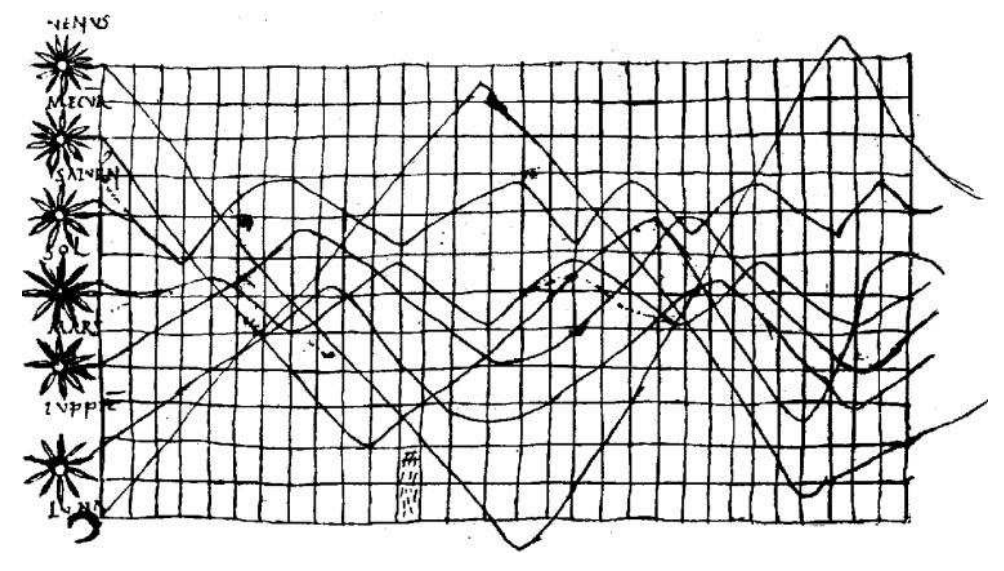
\includegraphics[keepaspectratio,width=\linewidth,height=\fullh / 3]
    {images/planetary-movements.png}
    \caption[Chart of Planetary Movements from the Tenth Century]{
        A chart created by an unknown astronomer in the tenth century depicting the movements of the seven most prominent planets. \imgcredit{Image extracted from \cite{BriefHistoryOfDataVis}. Original appearance in \cite{NoteOnTenthCenturyGraph}.}
    }
    \label{fig:PlanetaryMovements}
\end{figure}

\begin{figure}[tp]
    \centering
    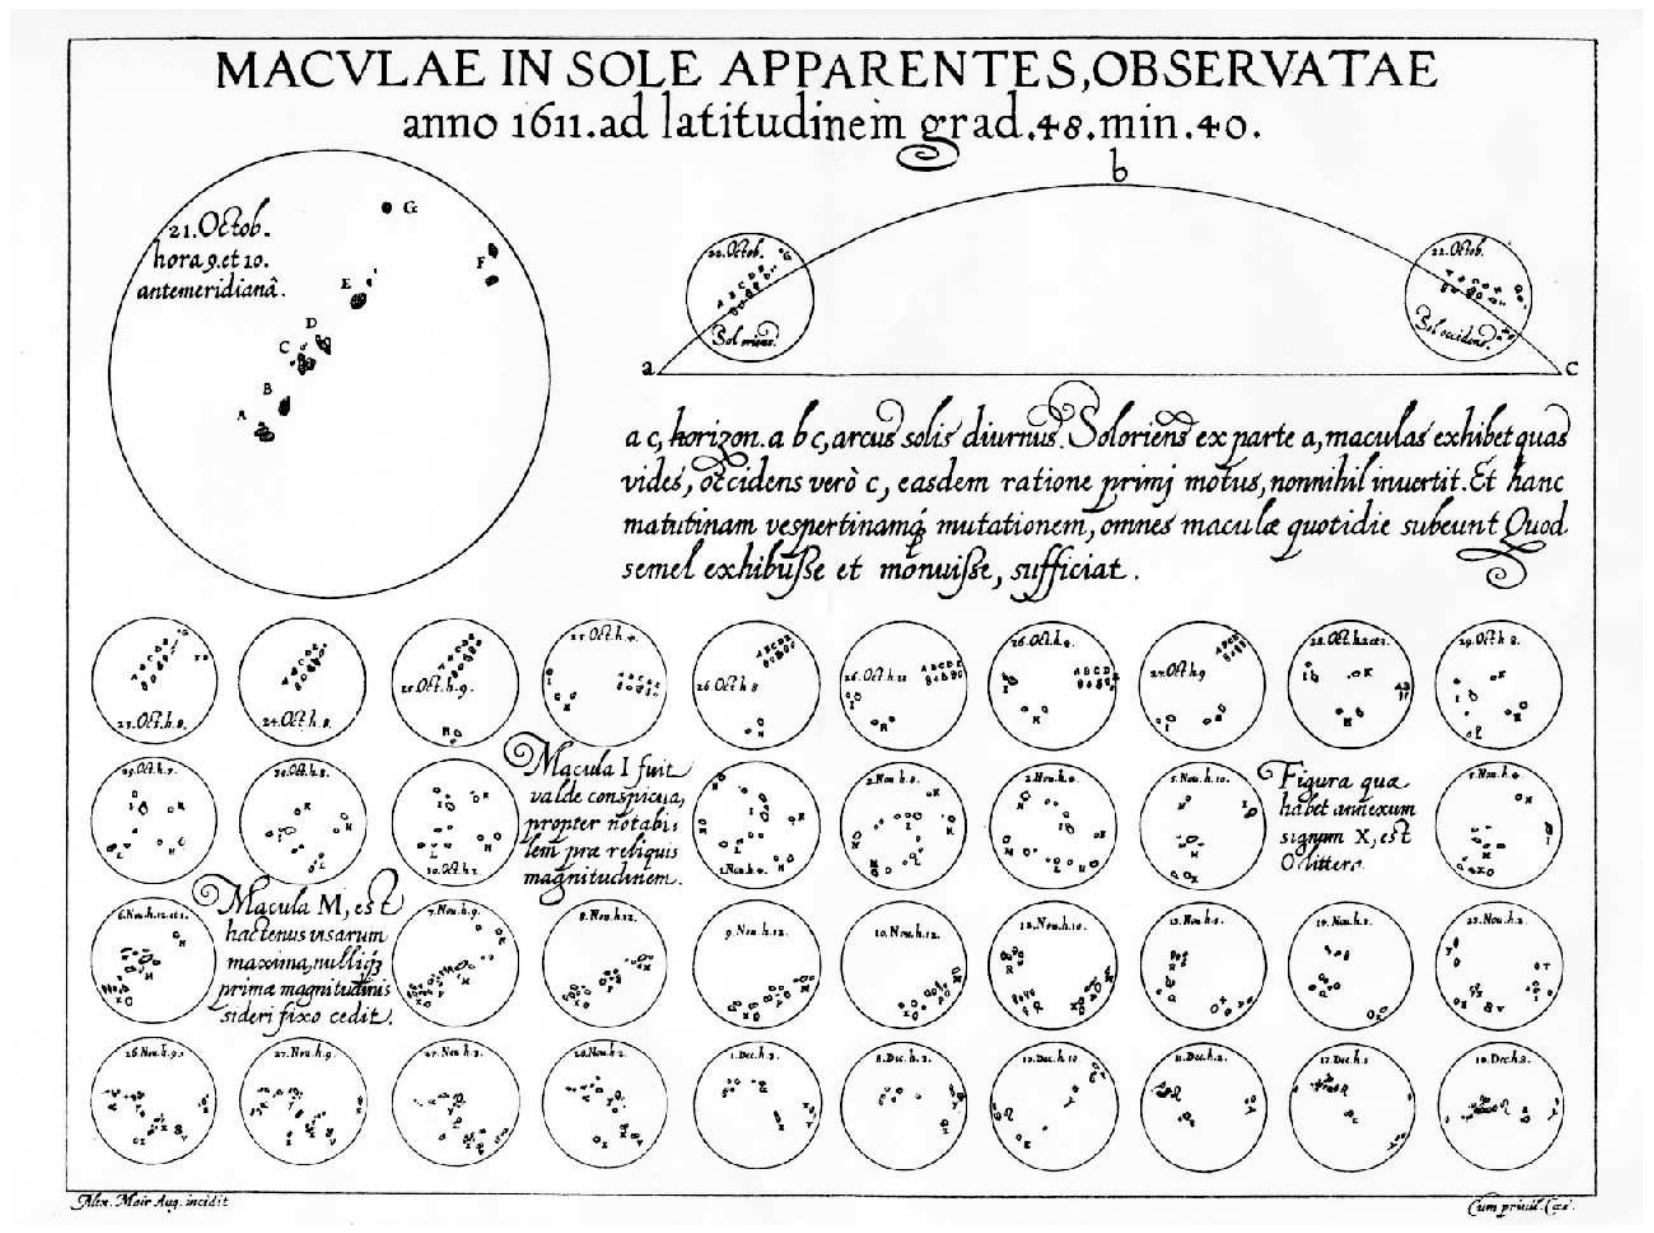
\includegraphics[keepaspectratio,width=\linewidth,height=\fullh / 3]
    {images/sunspot-changes.png}
    \caption[Chart of Changes in Sunspots from 1626]{
        This chart shows the observed changes in sunspots based on recordings of two months of data from 1611. It is the first occurrence of the principle later called "small multiples" by \cite{VisualDisplayOfQuantitativeInformation}. \imgcredit{Image extracted from \cite{BriefHistoryOfDataVis}. Original appearance in \cite{RosaUrsina}.}
    }
    \label{fig:SunspotChanges}
\end{figure}

\begin{figure}[tp]
    \centering
    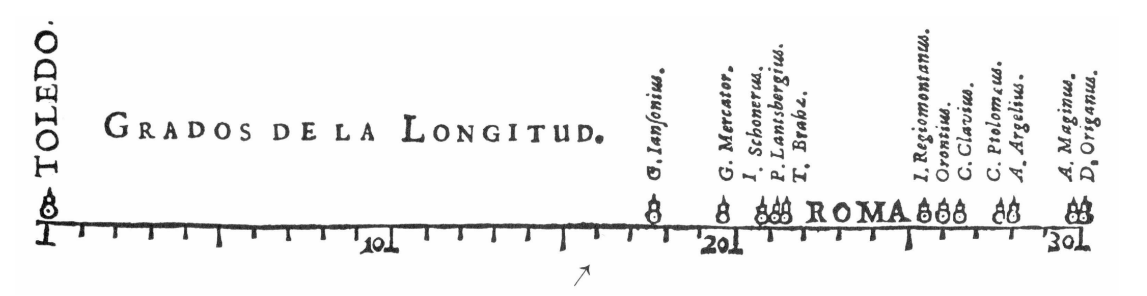
\includegraphics[keepaspectratio,width=\linewidth,height=\fullh / 3]
    {images/rome-toledo-longitude.png}
    \caption[Chart of Longitudinal Distance Determinations Between Toledo and Rome From 1644]{
        This chart compares the twelve known estimates in longitudinal distance between Rome and Toledo by various astronomers. The correct distance is marked by the arrow beneath. It is considered to be the first visual representation of statistical data. \imgcredit{Image extracted from\cite{BriefHistoryOfDataVis}. Original appearance in \cite{VisualExplanations}.}
    }
    \label{fig:RomeToledoLongitude}
\end{figure}

\begin{figure}[tp]
    \centering
    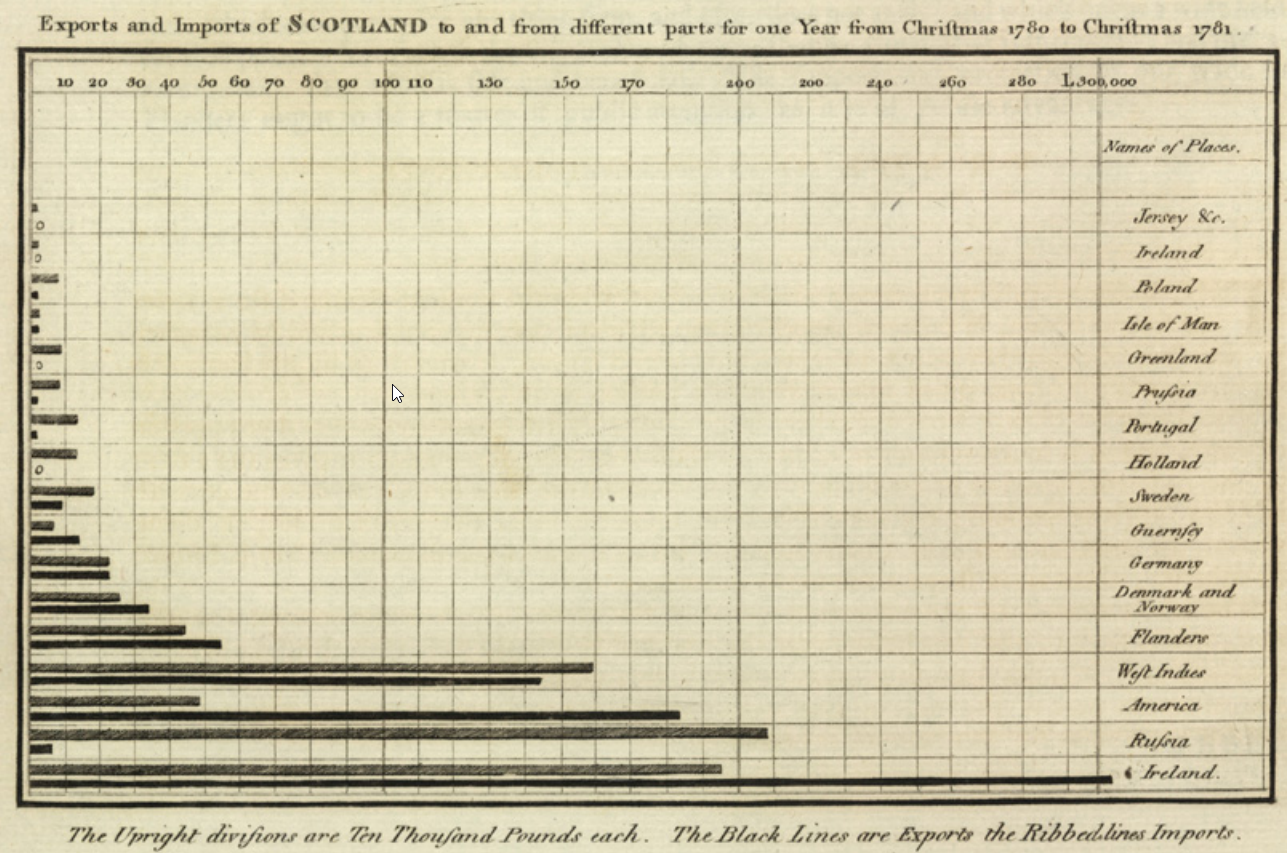
\includegraphics[keepaspectratio,width=\linewidth,height=\fullh / 3]
    {images/playfair-bar-chart.png}
    \caption[Chart of 1781 Exports and Imports of Scotland From 1786]{
        This chart shows the exports and imports from and to Scotland in 1781. It is considered to be the first published occurrence of a bar chart. \imgcredit{Image extracted from \cite{WilliamPlayfair}. Original appearance in \cite{CommercialAndPoliticalAtlas}.}
    }
    \label{fig:PlayfairBarChart}
\end{figure}

\begin{figure}[tp]
    \centering
    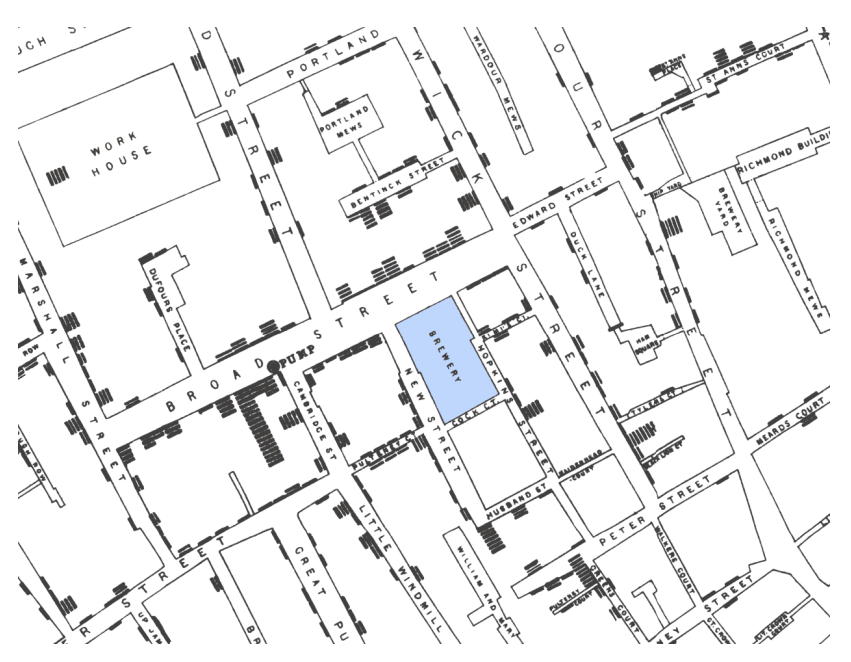
\includegraphics[keepaspectratio,width=\linewidth,height=\fullh / 3]
    {images/cholera-dot-map.png}
    \caption[Dot Map Plotting Cholera Deaths in London From 1855]{
        This iconic chart was created by Dr. John Snow to identify a clustering of cholera-related deaths near Broad Street in London. It was used to identify a contaminated water pump and to illustrate the waterborne nature of the disease. \imgcredit{Image extracted from \cite{IVISCourseNotes}. Original appearance in \cite{ModeOfCommunicationOfCholera}.}
    }
    \label{fig:CholeraDotMap}
\end{figure}

\section{Responsive Web Design}

\TODO{Define responsive web design} \TODO{Mention adapting to characteristics of consuming device} \TODO{Mention text wrapping} \TODO{Mention }

\TODO{Mention importance of responsive web design} \TODO{Add chart showing the rise of mobile devices} 

https://i.imgur.com/25ZpmBn.png

\section{Responsive Information Visualization}

\TODO{Mention necessity of responsive visualizations in context of responsive web design} \TODO{Mention visualizations being important blocks of content that can not be ignored when designing responsive web pages}

\TODO{Mention scalable vs responsive visualizations} \TODO{Mention responsive layout} \TODO{Mention responsive display density} \TODO{Mention responsive interaction}

\TODO{Mention the book Building responsive data visualizations for the web} \TODO{Mention focus on scalable visualizations rather than responsive visualizations}

\subsection{Responsive Visualization Patterns}

\TODO{Mention patterns in software development}
\TODO{Mention patterns in responsive web design}
\TODO{Mention patterns in visualizations}

\TODO{Mention patterns defined by Adler et. al}
\TODO{
    1. Rotating axis labels
    2. Removing axis ticks
    3. Shortening strings
    4. Flipping visualizations by 90 degrees
    5. Repositioning visual components
    6. Zooming
    7. Filtering
    8. Reducing data density
    9. Changing chart types
}

\TODO{Mention high-level actions for responsive adaptations of visualization as defined by Hoffswell et. all}
\TODO{Identified by analyzing 231 visualizations from various sources}
\TODO{
    1. No change
    2. Resizing visualizations
    3. Repositioning visual components
    4. Adding visual components
    5. Modifying visual components
    6. Removing visual components
}

\TODO{Mention patterns as defined by Kim et. al (2021 paper)}

\subsection{Responsive Visualization Examples}

\section{Information Visualization Libraries}

\subsection{Chartist}

\subsection{Highcharts}

\subsection{ECharts}

\subsection{...?}

\subsection{D3}

\TODO{Mention that D3 is successor of Protovis}

\subsection{D3FC}

\TODO{Mention the mixed HTML/SVG approach when it comes to layout}